

En esta sección se explica el diseño y funcionamiento del circuito diseñado para actuar como una carga electrónica controlada por voltaje. El propósito de este circuito, es ofrecer una condición de carga para la armadura del generador de manera que este ejerza un torque al motor DC, y que, además, esta carga pueda ser controlada desde el computador que está realizando el control del sistema. Se muestra a continuación el circuito ensamblado.



Para entender el funcionamiento del circuito, se debe saber que la parte más importante del mismo es el transistor BJT modelo TIP41C, ya que, este componente será el que disipe la mayor parte de la potencia eléctrica generada por el generador, por lo tanto, debe estar montado con un disipador térmico de buen tamaño. Además, se muestra el esquemático de la carga electrónica en la siguiente figura \ref{fig:cargaElec}.

\begin{figure}[H]
    \centering
    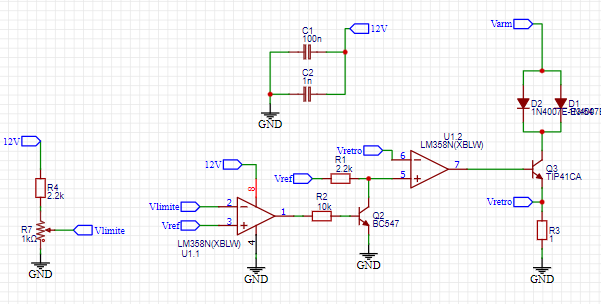
\includegraphics[width=0.75\linewidth]{img//cargaElectronica/cargaElec.jpg}
    \caption{Esquemático carga electrónica}
    \label{fig:cargaElec}
\end{figure}

Para realizar la función, el circuito se alimenta con 12 Volts, y el transistor se alimenta directamente de la armadura del motor, para el control de la corriente, el módulo recibe un voltaje de entrada, este voltaje de entrada es aplicado al Opamp (amplificador operacional), y este a su vez, lo aplica sobre la resistencia R3 del esquemático de la figura \ref{fig:cargaElec}, de esta manera, se produce una corriente igual a $\frac{Vcontrol}{R3}$, en muchas ocasiones se puede dejar R3 = 1 para que la corriente sea igual a Vcontrol, ademas, el transistor TIP41C es el encargado de proveer toda la corriente que pasar por la resistencia, por ende, el opamp termina siendo un controlador que no disipa mucha potencia (es importante que sea el modelo LM358). Por ultimo, la carga cuenta con 2 protecciones, 1) Un par de diodos D2 y D1 en la parte superior que impiden que se queme el transistor si es que se conecta en polaridad inversa la carga, y 2) el opamp 1.1 que impide que el voltaje Vcontrol aplicado a la resistencia R3 sea muy grande evitando que la carga pida mucha corriente, el valor de limite de corriente se puede ajustar a mano con el potenciómetro R7. Para garantizar un buen desempeño, se realizó una serie de pruebas a distintos voltajes y corrientes un con sensor de temperatura en el disipador para monitorear la temperatura del transistor TIP41C. Ver la tabla \ref{tab:datos}. Datos de la prueba: Tiempo de funcionamiento: 1 minuto, Temperatura ambiente: 28 grados celsius.

\begin{table}[H]
    \centering
    \caption{Temperaturas medidas (grados Celsius)}
    \begin{tabular}{|c|c|c|c|c|}
        \hline
        V, I & 0.2 A & 0.4 A & 0.6 A &  0.8 A\\
        \hline
        5 V & 28 & 29 & 31 & 30 \\
        \hline
        9 V & 29 & 31 & 33 & 34 \\
        \hline
        12 V & 32 & 33 & 38 & 37 \\
        \hline
    \end{tabular}
    \label{tab:datos}
\end{table}


